\begin{abstract}
A common pessimistic argument holds that autoregressive language models suffer exponential decay in correctness over long outputs: if each token has independent error probability $e$, then $(1-e)^n \to 0$ as $n$ grows. The argument is clean to state and widely cited. It is also brittle, and three lines of recent empirical work make the cracks visible. The first is that only a small minority of tokens genuinely depends on long-range context or carries a decision---under $10\%$ in a direct measurement of long-range dependence on one natural-text corpus, while in reasoning traces more than half of tokens are nearly deterministic; the rest get more predictable, not less, as context accumulates. The second is geometric: analyses of LLM embeddings report stratified low-dimensional structure, which on our reading keeps a model inside one semantic region even when individual tokens slip. The third concerns what happens when models do err on the consequential tokens: on reasoning benchmarks, sampling several answers and taking the majority recovers substantial accuracy, which on our reading means those errors are often idiosyncratic across samples rather than systematic. Pulling these together gives a two-rate model, $P(\text{correct}) \approx (1-e_{\text{key}})^k \cdot (1-e_{\text{non}})^{n-k}$, in which, we hypothesize, $k$ scales sublinearly with $n$ and $e_{\text{non}}$ approaches zero with sufficient context. The predicted decay is, at worst, stretched-exponential; often power-law; and when $k$ saturates at some task-specific $k_{\max}$, constant in $n$. A number of recent capabilities---learned compression of the key-value cache, $128$K-token retrieval on consumer GPUs, self-consistency gains on reasoning benchmarks---then read as consequences of one structural fact rather than independent engineering wins: long-context reliability hinges on a handful of decision points, not on uniform per-token accuracy. We also mark where the argument stops: when the number of decisions grows with the task, as in long-horizon agentic work, the same model predicts the roughly exponential decline with task length that agent evaluations report.
\end{abstract}

\section{Introduction}
\label{sec:intro}

Autoregressive language models, the argument goes, are doomed for long outputs. If each token has even a $1\%$ error rate then a $100$-token chain is correct only $(0.99)^{100} \approx 37\%$ of the time, and longer chains decay exponentially toward zero \citep{lecun2023why}; \citet{dziri2023faith} prove the step-level analogue for compositional tasks, where independent per-step errors drive the probability of a correct final answer down exponentially in the number of steps. The argument is clean, and it has been used to predict a hard ceiling on what autoregressive systems can do.

What modern LLMs actually do is harder to square with this picture. Multi-page outputs hold together. Later tokens sometimes revise earlier interpretations, as the examples collected in the inner-monologue literature show \citep{gwern2023inner}, which is difficult to reconcile with monotonically increasing error. The attention patterns are lopsided: in a $128$K-token context, attention computed from only the top-$k$ critical tokens approaches full attention once $k$ is in the low hundreds \citep{liu2024retrieval}, and fewer than $10\%$ of tokens in a natural-text corpus (GovReport) gain substantially---more than $2$ nats of log-probability---from the full context over a truncated short context \citep{fang2024what}. A smaller base model paired with the right test-time-compute strategy can outperform a model roughly $14\times$ its size on reasoning problems where the smaller model already has a non-trivial success rate \citep{snell2024scaling}. None of this is consistent with uniform per-token error.

Our reading is that the independent-error model fails because it averages over a heterogeneous population of tokens. A small fraction---key tokens---carry the load of long-range dependency and global coherence. The rest are constrained by local syntax and the accumulating context, and their error rate goes to zero rather than to a constant. Three threads of recent work make this concrete: \citet{fang2024what} on which tokens actually need long context, \citet{li2025unraveling} on the stratified-manifold organization of embeddings, and \citet{wang2023self} on how diverse correct reasoning paths agree on one final answer under sampling. Combined, they produce a refined model:
\begin{equation}
\label{eq:two-rate}
P(\text{correct}) \approx (1-e_{\text{key}})^k \cdot (1-e_{\text{non}})^{n-k},
\end{equation}
where $k$ is the number of key tokens, $e_{\text{key}}$ their error rate, and $e_{\text{non}}$ the much lower error rate for the remaining $n-k$. If $k$ scales sublinearly with $n$---logarithmically, as a fractional power, or saturating at some $k_{\max}$---and $e_{\text{non}} \to 0$ with context, the predicted decay is far gentler than $(1-e)^n$.

\paragraph{Contributions.}
(1)~A two-rate error model that distinguishes key from non-key tokens and makes the dependence on $k(n)$ explicit (\S\ref{sec:framework}). (2)~A synthesis of evidence from three recent research streams---attention sparsity, embedding geometry, and ensemble convergence---that supports each component of the model (\S\ref{sec:evidence}). (3)~An accounting of how this framework reframes existing systems-level results (anchor compression, retrieval-augmented attention, self-consistency, tool integration) as predictable consequences of a single structural fact rather than independent engineering wins (\S\ref{sec:implications}).

\section{Related Work}
\label{sec:related}

\paragraph{Error compounding.}
The exposure-bias problem is old. \citet{bengio2015scheduled} identified its mechanism: a model trained to predict each token from the true previous token must, at inference time, condition on its own generated tokens, so errors can accumulate along the generated sequence. \citet{lecun2023why} restated the worry for autoregressive LLMs in the now-familiar form---if each token has error probability $e$, sequence-level correctness decays as $(1-e)^n$. The bound is tight when independence really holds, and loose otherwise; transformers attending backward over their own output is exactly the case where it goes loose, and the self-correction examples collected in \citet{gwern2023inner}---error rates that \emph{decrease} at certain points in a sequence---are hard to reconcile with strict monotonic accumulation. We keep the per-token decomposition but partition tokens by their long-range dependency. The step-level version of the worry has since acquired data of its own: \citet{kwa2025measuring} find that agent success falls off smoothly with the human time a task takes, \citet{ord2025halflife} argues that a constant hazard rate per minute of human task time---exponential decay in task length---fits those data about as well as METR's own curve, while calling the evidence so far only suggestive, and \citet{sinha2025illusion} find that per-step execution accuracy degrades along long horizons partly because models condition on their own earlier mistakes. We return to how these step-level results relate to the token-level argument in \S\ref{sec:limitations}.

\paragraph{Long-context utilization.}
\citet{liu2023lost} documented the lost-in-the-middle effect---models often perform best when the relevant material sits near the beginning or end of the prompt and worst when it sits in the middle. The same skew was given a sharper edge by \citet{fang2024what}, whose long-short difference (LSD) metric finds fewer than $10\%$ of tokens in a natural corpus (GovReport) scoring LSD$>2$---that is, predicted materially better with the full context than with a truncated short context (their LongPPL experiments truncate to the preceding $4{,}096$ tokens; the window behind this particular figure is not stated). \citet{liu2024retrieval} show that in a $128$K-token context the attention output computed from only the top-$k$ critical tokens approaches full attention once $k$ is in the low hundreds, and exploit this to serve $128$K-token contexts for 8B-parameter models on a single 24\,GB consumer GPU. Anchor compression \citep{pang2024anchor}---Llama2-7B continually pre-trained to fold each sequence into an anchor token---cuts the keys/values cache of cached five-shot demonstrations by up to $99\%$ on short question-answering benchmarks, at an average accuracy cost of about $1.5\%$. Each of these papers treats sparsity as an empirical fact about a particular system; we read them as direct evidence for $k \ll n$.

\paragraph{Embedding geometry.}
\citet{li2025unraveling} probed LLM embedding spaces with sparse mixture-of-experts and report a stratified-manifold structure in static embeddings of models up to 1.5B parameters: a union of low-dimensional submanifolds aligned with the source of the data. \citet{robinson2025token}'s fiber-bundle hypothesis test flags tokens whose embedding neighborhoods violate the local-smoothness assumption; they argue, via a theorem on how such singularities propagate to the output, that of two semantically equivalent prompts the one containing a flagged token will likely receive the less stable response---an implication they leave to future experiments. \citet{viswanathan2024geometry} link intrinsic dimensionality to prediction loss: across prompts, those whose token representations occupy lower-dimensional point clouds have lower average surprisal. And \citet{gao2024insights} find that a probe can almost perfectly locate the target key-value pair from the model's hidden states even when the generated answer is wrong (on multi-document question answering, probing accuracy is consistently above generation accuracy). On our reading, compartmentalized representations, irregular embedding neighborhoods, and lower-dimensional states under confidence are what let a model absorb small token-level slips without breaking coherence at the semantic level.

\paragraph{Ensemble reasoning.}
Self-consistency, in \citet{wang2023self}'s formulation, is almost embarrassingly simple: sample multiple reasoning paths, take the majority answer. The gain was $+17.9$ points on GSM8K, with no retraining. Tree-of-Thoughts \citep{yao2023tree} extends the idea with structured tree search over intermediate thoughts, each branch self-evaluated before expansion, and pulls GPT-4 on Game-of-24 from $4\%$ to $74\%$. On our reading, the pattern these methods exploit is that errors on reasoning-heavy questions tend to be idiosyncratic across samples (different paths fail at different junctions) while errors on knowledge-gap questions tend to be systematic (every sample fails the same way), so ensembles should help in the first case and not in the second. Neither paper tests this split, and the evidence is mixed: in the Tree-of-Thoughts experiments, majority voting over $100$ chain-of-thought samples lifts GPT-4 on Game of 24 only from $4\%$ to $9\%$. Where ensembles do help, the size of the effect is the part the independent-error model cannot absorb. If errors compounded uniformly, multiple samples would yield multiple failures, not a more accurate mode.

\paragraph{Decision-point tokens in reasoning.}
Three studies not discussed in the first version of this paper locate the same structure inside reasoning traces rather than in long-context prediction. \citet{bigelow2025forking}, re-sampling GPT-3.5 generations token by token on seven tasks, find \emph{forking tokens}---sometimes a single punctuation mark---where re-sampling sends the outcome somewhere very different, with abrupt shifts in up to $63\%$ of examples depending on the task; their survival analysis also finds smaller hazards accumulating gradually along most paths. \citet{lin2024critical} identify, by rollout sampling, a \emph{critical token} in each incorrect reasoning trajectory of Llama-3-8B on GSM8K and MATH, and find that forcing a different token at that one position recovers the correct answer in about $30\%$ of single re-samples and in over $90\%$ of cases within $64$. \citet{wang2025beyond8020} find that token entropy in chain-of-thought generation is sharply skewed---over half of tokens fall below $0.01$---that the high-entropy minority (they take the top $20\%$) acts as forks between reasoning paths, and that restricting policy-gradient updates to that top $20\%$ matches full-gradient reinforcement learning on Qwen3-8B and exceeds it on the 14B and 32B models (+11.0 points on AIME'25 for 32B). The criteria differ---entropy at generation time, the effect of re-sampling, dependence on distant context---but they point the same way: the outcome turns on a minority of positions.

\section{Theoretical Framework}
\label{sec:framework}

We develop the two-rate model in three stages: the partition of tokens into key and non-key, the manifold dynamics that structure error correlation, and the redundancy gain that ensemble methods extract.

\subsection{Two-Rate Error Model}

The independent-error argument assumes every token carries equal weight in the failure probability. It does not. Key tokens are the ones whose correctness genuinely depends on long-range context or global knowledge---factual claims, logical operators, points of co-reference, transitions between topics. Non-key tokens are governed by local regularity: syntax, frequent collocations, content already established by the surrounding text. Their error rate is small and decreases as more context accumulates.

In a sequence of length $n$, let $k$ count the key tokens. A direct estimate of $k/n$ for natural text comes from the long-short-difference analysis of \citet{fang2024what}: fewer than $10\%$ of GovReport tokens gain more than $2$ nats of log-probability from the full context relative to a truncated short context. The fraction depends on the short-window length $K$ used to define ``long range,'' so we write it as $\alpha_K$; adversarial-perturbation studies, which ask a different question, land in the same order of magnitude \citep{jin2020textfooler}. We hypothesize that $k$ grows sublinearly with $n$, possibly saturating at a task-specific $k_{\max}$: even a book-length argument operates within a finite knowledge frame requiring a bounded number of critical decisions. With per-token error rates $e_{\text{key}}$ (large) and $e_{\text{non}}$ (small, decreasing in context), Eq.~\ref{eq:two-rate} gives three regimes:

\begin{enumerate}
\setlength{\itemsep}{1pt}
\item \textbf{Logarithmic key-token growth} ($k \sim \log n$): polynomial decay $n^{-c}$, much slower than exponential.
\item \textbf{Fractional-power growth} ($k \sim \sqrt{n}$): stretched-exponential decay.
\item \textbf{Saturating} ($k \to k_{\max}$): reliability becomes constant in $n$ once the key facts are committed.
\end{enumerate}

Two conditions are doing the work here, and both should be explicit. First, the regimes describe the key-token factor; the non-key factor $(1-e_{\text{non}})^{n-k}$ stays bounded away from zero only if the non-key error rates are summable, $\sum_i e_{\text{non}}(i) < \infty$---for instance $e_{\text{non}}(i) = O(i^{-(1+\delta)})$ for some $\delta > 0$. A constant $e_{\text{non}}$, however small, makes the non-key factor itself exponential in $n$ and the argument collapses; the claim that $e_{\text{non}} \to 0$ with context is therefore load-bearing, not decorative, and \S\ref{sec:evidence} collects the evidence for it. Second, with $k = c \ln n$ the key factor is $(1-e_{\text{key}})^{c \ln n} = n^{-c \ln(1/(1-e_{\text{key}}))}$, a power law whose exponent is small when $e_{\text{key}}$ is; and the saturating regime needs both $k \to k_{\max}$ and the summability condition. Figure~\ref{fig:regimes} plots the four curves for illustrative parameters.

\begin{figure}[t]
\centering
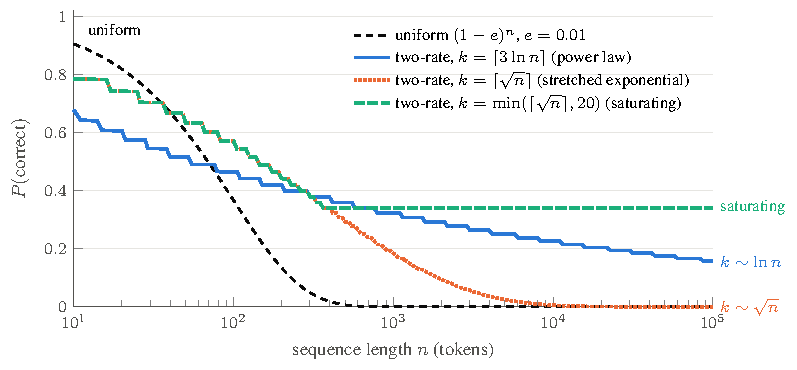
\includegraphics[width=0.8\linewidth]{fig1_decay_regimes}
\caption{Sequence-level correctness under the uniform model $(1-e)^n$ and under the two-rate model of Eq.~\ref{eq:two-rate} in its three regimes. Illustrative parameters: $e = 0.01$; $e_{\text{key}} = 0.05$; $e_{\text{non}}(i) = 0.02\, i^{-1.5}$ (summable); $k = \lceil 3 \ln n \rceil$, $k = \lceil \sqrt{n} \rceil$, and $k = \min(\lceil \sqrt{n} \rceil, 20)$. The curves are the functional forms the argument predicts, not fits to data.}
\label{fig:regimes}
\end{figure}

The third regime is the strange one. \citet{pang2024anchor} continually pre-train Llama2-7B to compress each sequence into a single anchor token; on five-shot question-answering benchmarks this discards up to $99\%$ of the demonstrations' keys/values cache at an average accuracy cost of about $1.5\%$. On our reading, a model that can be trained to carry each span forward in one position is consistent with a bounded number of load-bearing positions per span, and hard to square with a view in which every token carries equal weight.

\subsection{Stratified Manifold and Error Correlation}

The $(1-e)^n$ form also assumes errors are independent across positions. They are not. If the embedding space is stratified, as \citet{li2025unraveling} report for static input embeddings, we expect that structure to introduce correlation between errors; we model the dynamics as follows. Treat the model's hidden state as moving along a manifold $M_C$ determined by the prevailing context. Most errors are minor---a synonym substitution, a grammatical slip, a momentary wobble that stays on $M_C$ and has no downstream effect. Disruptive errors are different: a key-token mistake jumps the trajectory onto a different manifold $M_{C'}$, after which subsequent tokens cohere with the wrong commitment. The result is a fluent-but-wrong continuation. Errors cluster rather than scatter.

Two consequences follow, and they are separate. The first needs no correlation at all: whatever the dependence between positions, the union bound gives
\begin{equation}
\label{eq:union}
P(\text{any disruptive error}) \le k\, e_{\text{key}},
\end{equation}
to be compared with the uniform model's $1-(1-e)^n \approx n e$ for small $e$. The ratio of the two is $k/n$: with fewer than a tenth of positions carrying key decisions, the failure budget shrinks by at least that factor before any correlation is invoked. The second consequence is the correlation itself. When key-token failures co-occur---a wrong commitment early makes later positions cohere with it rather than fail independently---the probability of at least one failure sits \emph{below} the independent-errors value $1-(1-e_{\text{key}})^k$, because the same failure mass is concentrated in fewer sequences. Clustering does not make failures rarer per position; it makes them rarer per sequence. The manifold structure also offers a reading of the gap \citet{gao2024insights} document: intermediate layers encode where the needed information sits even when the generated answer is wrong. On our reading, the hidden-state trajectory can remain on the correct manifold while the output does not; the authors attribute the gap to positional bias and late extraction.

\subsection{Self-Consistency and Redundancy Gain}

When key-token errors are idiosyncratic across samples---different paths fail at different junctions---majority-vote ensembles can recover the correct answer. For $m$ samples with error correlation $\rho$, write the effective error rate at a key decision as
\begin{equation}
\label{eq:ensemble}
e_{\text{key}}^{\text{(eff)}} = f(\rho, m)\, e_{\text{key}},
\end{equation}
where $f \to 1$ at $\rho = 1$ (perfect correlation: every sample fails the same way, no gain). At $\rho = 0$ the value of $f$ depends on how the samples are combined. With an oracle verifier that accepts any correct sample (Pass@$m$), $f = e_{\text{key}}^{m-1}$. With majority voting---which is what self-consistency actually does---the effective error is the binomial tail $P[\mathrm{Bin}(m, e_{\text{key}}) \ge \lceil m/2 \rceil]$, which by Hoeffding's inequality is at most $\exp\!\big(-2m(\tfrac12 - e_{\text{key}})^2\big)$ whenever $e_{\text{key}} < \tfrac12$: still exponential in $m$, but at a rate set by the margin below one half rather than by $e_{\text{key}}$ itself. The condition $e_{\text{key}} < \tfrac12$ is not a technicality. It says majority voting can only help at decisions the model already gets right more often than not, which, on our reading, is why it should fail on knowledge-gap errors (\S\ref{sec:related}), where every sample inherits the same wrong answer. On our reading, Wang et al.'s results \citep{wang2023self} sit closer to the $\rho = 0$ regime than to $\rho = 1$ (they do not measure error correlation): a method that adds no parameters and no training data lifts GSM8K accuracy by $17.9$ points, and the gain is robust to temperature, top-$k$, and nucleus settings.

\citet{costello2025think} observe that iterative self-training raises Pass@1 while Pass@$k$ remains relatively stable. On our reading, the headroom from sampling more (Pass@$k$ minus Pass@1, the most an oracle selector could gain) shrinks as probability mass concentrates on correct paths---the authors themselves describe the model as converging ``on a narrower set of high-probability outputs''---so ensembles help only while the model's spread of guesses still straddles the right region.

\section{Empirical Evidence}
\label{sec:evidence}

Three predictions, three lines of evidence. The framework says $k/n$ is small and stable; that token errors correlate via manifold geometry; and that correct reasoning paths converge while incorrect ones diverge. The supporting work for each comes from a different methodology, which is what makes the convergence interesting.

\subsection{Key-Token Sparsity}

The most direct measurement is \citet{fang2024what}'s long-short difference. A token counts as key if the full context improves its log-likelihood by more than $2$ nats over a truncated window ($4{,}096$ tokens in their LongPPL experiments) and the token remains predictable under the full context; on GovReport, fewer than $10\%$ of tokens clear even the first criterion. Perplexity restricted to those tokens (LongPPL) correlates with LongBench performance at Pearson $-0.96$ across the models they evaluate, where ordinary perplexity over all tokens correlates at $-0.18$; and on a retrieval task where the answer tokens are known in advance, perplexity on the non-answer tokens carries almost no signal at all. Adversarial robustness work, working from the opposite direction, lands in the same order of magnitude. TextFooler \citep{jin2020textfooler}, catalogued with related attacks in \citet{morris2022textattack}, drives classifier accuracy below $15\%$ on every dataset except fake-news detection (below $10\%$ for most model--dataset pairs) by swapping $3.5\%$--$22\%$ of words depending on task and target model---$3.5\%$--$6\%$ on long IMDB reviews, about $14\%$--$19\%$ on short entailment pairs---and its ablation (BERT on MR, AG, and SNLI) shows that choosing \emph{which} words to perturb is what does the work: with the importance ranking removed and words chosen at random, after-attack accuracy rises by more than $45$ points. A minority of positions carries the decision whichever way one measures it; the exact fraction depends on the criterion, and we return to that dependence in \S\ref{sec:limitations}.

The systems-level corollary is sharp. \citet{liu2024retrieval} serve $128$K-token contexts for 8B models on a single consumer GPU by attending, at each decoding step, only to the $100$ keys retrieved by an attention-aware nearest-neighbour index plus $640$ fixed initial and recent tokens, with accuracy close to full attention. Anchor-LLM \citep{pang2024anchor}, after continual pre-training, compresses each cached demonstration into a single anchor token, cutting the keys/values cache by up to $99\%$ on short question-answering benchmarks at an average accuracy cost of about $1.5\%$. Neither result would be expected if token importance were uniform.

\subsection{Stratified Manifold Structure}

\citet{li2025unraveling}'s sparse-MoE probe of frozen LLM embeddings (models up to 1.5B parameters) finds a union of low-dimensional manifolds aligned with data source (movie and product reviews, tweets, news), with measurably different intrinsic dimension across regions. \citet{robinson2025token}'s fiber-bundle test identifies irregular-neighborhood tokens in the input-embedding spaces of four open LLMs and argues that prompts containing them will likely yield less stable responses (failing to reject regularity at a token is, in their words, uninformative). On our reading, irregular tokens are candidate manifold junctions---points where a small input change could move the trajectory between regions, as the authors themselves illustrate with tokens such as `*' that join distinct usages; whether they coincide with the key tokens of our partition is untested, and most flagged tokens are word-initial pieces and word fragments.

\citet{viswanathan2024geometry} link this to confidence: prompts that elicit low-intrinsic-dimensional representations correlate with lower prediction loss. On our reading, if confident prediction goes with a lower-dimensional state, context that progressively constrains the state should push $e_{\text{non}}$ down rather than leave it constant---a within-sequence prediction the paper does not test.

\citet{gao2024insights} train layer-wise probes that locate the target information in intermediate representations---almost perfectly on key-value retrieval---even when the LLM's generated answer is wrong, a ``know but don't tell'' gap between probing accuracy and generation accuracy that holds across positions and across models. The location of the needed information was encoded internally; the failure was in using it. On our reading this is the manifold-stays-correct behavior our framework predicts; the authors explain it by positional bias, noting that the later a layer locates the information, the lower the generation accuracy.

\subsection{Convergent Reasoning Paths}

\citet{wang2023self} showed that self-consistency lifts GSM8K by $17.9$ points and SVAMP by $11.0$ (GPT-3 code-davinci-002), with no model change. The mechanism, on our reading, is that correct paths---diverse as they are---converge on one final answer while incorrect ones scatter across many, so majority voting picks out the mode. \citet{yao2023tree}'s Tree-of-Thoughts moves GPT-4 on Game-of-24 from $4\%$ to $74\%$ by breadth-first search over intermediate steps, keeping at each step the five partial solutions the model itself rates most promising; their error analysis finds that about $60\%$ of chain-of-thought samples have already failed after the first step. Why should sampling help on some questions and not others? Our conjecture, which no cited study tests, is that knowledge gaps produce systematic errors (every sample fails the same way) while reasoning slips produce idiosyncratic ones (samples fail differently), and ensembling extracts no signal in the former regime. The Game-of-24 case, where majority voting barely helps, shows that reasoning errors can be systematic too. The framework's two error rates accommodate both: $e_{\text{key}}$ rises uniformly when the model lacks the relevant fact or the relevant strategy, and ensembling cannot help.

A summary of how the systems-level results map onto the framework's three pillars appears in Appendix~\ref{app:systems}.

\section{Practical Implications}
\label{sec:implications}

The framework is not just a description of why $(1-e)^n$ is wrong. It also predicts where computation should go, how context should be managed, and what to evaluate.

\paragraph{Sparse attention and context compression.}
If $k \ll n$, attention does not need to be dense. \citet{pang2024anchor}'s anchor compression and \citet{liu2024retrieval}'s top-$k$ attention are the existing demonstrations; \citet{wu2024tokenselect}'s dynamic KV-cache selection is another point on the same curve. These methods stop being clever tricks and become predictable: dense attention pays a quadratic cost to recover a sparse signal.

\paragraph{Targeted compute at decision points.}
If errors concentrate at manifold transitions, compute should too. \citet{moshkov2025aimo}'s tool-integrated reasoning lets the model decide where to hand off to Python: it emits code blocks where it chooses---its training data favour code that buys a real shortcut, such as numeric solving or exhaustive search---under a code-execution cap stated in the prompt (randomized between one and eight per problem in training), rather than computing everywhere. \citet{schuster2022calm}'s Confident Adaptive Language Modeling commits to a prediction at an earlier transformer layer when the model's intermediate confidence is high enough, reporting up to $3\times$ wall-clock speedup on text-generation tasks while preserving output quality. The adaptive-temperature sampling of \citet{zhu2024hotorcold} raises the temperature at the first token of each code block---where their loss analysis finds hard-to-predict tokens concentrate---and lowers it elsewhere. Three different prescriptions, one underlying instruction: spend cycles where the manifold is about to fork.

\paragraph{Strategic ensembles.}
\citet{wang2023self}'s self-consistency bets on correct paths converging on a shared answer, and \citet{moshkov2025aimo}'s GenSelect targets the gap it leaves---problems a model sometimes solves but not by majority---by comparing sampled solutions and picking the most promising one. \citet{yao2023tree}'s tree search instead exploits the model's ability to evaluate partial solutions at intermediate decision points. On our reading, the framework explains why such methods work and predicts when they will not: when errors are systematic rather than idiosyncratic, as in knowledge-retrieval tasks where every sample inherits the same gap.

\paragraph{Evaluation aligned with key tokens.}
Plain perplexity averages over a population the model is trying to handle separately, which is why it underperforms as a predictor. \citet{fang2024what}'s LongPPL restricts perplexity to key tokens and lifts the correlation with LongBench performance to $r = -0.96$, from $-0.18$ for ordinary perplexity. \citet{costello2025think}'s self-improvement curves---Pass@1 rising round by round while Pass@$k$ holds---show that single-sample accuracy and coverage can move independently, so evaluations should report both.

A more speculative implication---modular reasoning architectures that route by manifold region, building on the self-training-over-scale results of \citet{costello2025think}---we defer to Appendix~\ref{app:arch}.

\section{Limitations}
\label{sec:limitations}

The framework is a synthesis, not a derivation. Five cautions belong on record. The two-rate model is descriptive: $k$, $e_{\text{key}}$, and $e_{\text{non}}$ are observable in principle but not yet jointly measured on a single benchmark, so the predicted decay regimes are arguments from supporting evidence rather than fitted curves. The manifold-structure account leans on \citet{li2025unraveling} and \citet{robinson2025token} for direct geometric evidence; both are recent, and replication on larger model scales would tighten the claim. The convergent-paths claim relies on a soft distinction between idiosyncratic and systematic errors; we have no quantitative criterion for separating the two in advance, only the post-hoc observation that ensemble methods help in the former regime and not in the latter, and the distinction itself is our conjecture rather than a result any cited study tests.

The fourth caution deserves more weight than the first version of this paper gave it. The token-level argument says reliability is governed by the number of key decisions, $k$; it says nothing about how $k$ grows with the \emph{task}. For long-horizon agentic work the answer appears to be: linearly. \citet{kwa2025measuring} find that agent success falls off smoothly with the human time a task takes, and \citet{ord2025halflife} argues that a constant hazard rate---exponential decay in task length---fits those data about as well as METR's own curve, while calling the evidence so far only suggestive. If that reading holds, it is not a contradiction of Eq.~\ref{eq:two-rate}; it is Eq.~\ref{eq:two-rate} in the regime where each additional subtask brings its own key decisions, so $k \propto n_{\text{steps}}$ and the decay is exponential in $k$. What the two-rate model rules out is exponential decay in \emph{tokens} at a fixed decision count, not exponential decay in decisions. \citet{sinha2025illusion} supply a mechanism that sits between the two levels: per-step execution accuracy degrades along a long horizon partly because the model conditions on its own earlier mistakes---the fluent-but-wrong continuation of \S\ref{sec:framework} playing out across steps---and models trained to reason before acting largely escape it. The bridge from token-level to step-level decay should start there.

Finally, $k/n$ is criterion-dependent. The long-context estimate is under $10\%$ of GovReport tokens against a truncated window whose length the source does not state for that figure \citep{fang2024what}; in reasoning traces, over half of tokens are near-deterministic, and the top-$20\%$ entropy cutoff of \citet{wang2025beyond8020} is a design choice rather than a measured fraction; an importance-ranked synonym attack must change $3.5\%$ to $22\%$ of words to flip a text classifier \citep{jin2020textfooler}. A direct measurement of $k(n)$ would fix the short-window length $K$, compute the cumulative count of LSD-key tokens at $n \in \{1, 2, 4, 8, 16\}$K on a fixed corpus, and fit $k \propto n^{b}$: sublinear growth means $b < 1$ with a confidence interval excluding $1$. A constant fraction ($b \approx 1$) would falsify the sublinear hypothesis under that criterion and leave only the slower exponential $(1-e_{\text{key}})^{\alpha_K n}$. We regard this as the most important open test of the framework.

\section{Conclusion}
\label{sec:conclusion}

The independent-error argument was always going to fail in one of two places. Either some tokens would matter more than others, breaking the per-token uniformity; or errors would correlate, breaking the independence. The evidence suggests both fail at once: in a direct measurement on one natural-text corpus, under a tenth of tokens carry the long-range dependency; embedding studies report stratified structure that, on our reading, compartmentalizes errors; and ensemble methods extract gains that a uniform-error model would not predict.

The two-rate model in Eq.~\ref{eq:two-rate} is a small change to the algebra and a large change to the predicted behavior. Reliability depends on $k$ key decisions, not on $n$ tokens; and, we hypothesize, $k$ scales sublinearly, often saturating. Modern LLMs hold coherence across thousands of tokens not because the underlying $(1-e)^n$ is being beaten by clever engineering, but because $(1-e)^n$ was the wrong functional form to begin with.

The systems-level consequences are already visible. Anchor compression, retrieval-augmented attention, tool-integrated reasoning, and self-consistency all gain explanatory unity once they are read as instances of a single principle: identify where the manifold forks, and put the compute there. Future work should run the $k(n)$ measurement laid out in \S\ref{sec:limitations}, derive tighter bounds from attention-pattern statistics rather than from heuristic union bounds, and connect token-level decay to the reasoning-step decay that bears more directly on agentic systems. Two companion papers take the next steps: \citet{arbuzov2026architecture} asks what the recurring key-decision failures are inside a bounded deployment domain and how the budget of interventions needed to cover them grows, and a third paper surveys how production systems already patch those failures outside the model weights.

\bibliographystyle{plainnat}
\bibliography{references}

\appendix

\section{Architectural Implications: Modular Reasoning}
\label{app:arch}

The stratified-manifold view suggests an architectural prescription the main body only gestures at: instead of scaling monolithic models, route reasoning subtasks to specialized models aligned with manifold regions. The clearest existing evidence comes from self-training-over-scale work. \citet{costello2025think}'s Think-Prune-Train (TPT) pipeline shows that models iteratively fine-tuned on their own correctness-pruned reasoning traces can close much of the gap to far larger ones on GSM8K---Gemma2-2B from $41.9\%$ to $57.6\%$ Pass@1, Gemma2-9B to $82\%$ (above LLaMA-3.1-70B-Instruct's $78\%$, a model about $8\times$ larger), and LLaMA-3.1-70B itself to $91\%$ (above GPT-4o's $82\%$). Whether explicit routing on top of these self-trained smaller models compounds the gains, or runs into a ceiling once the routed-to manifold is itself stratified, is the natural next question; we are not aware of a definitive empirical answer.

The pattern across these systems is consistent. Fitting the manifold beats expanding the parameter count, when the task population is narrow enough that the manifold is well-defined. The open question is how broad a domain a single specialized model can cover before its internal stratification reasserts itself and the routing problem reappears one level down. We do not attempt to settle that here; it is a question for empirical work that systematically varies routing granularity.

\section{Extended Case Studies in Advanced Reasoning Systems}
\label{app:systems}

The main body summarizes the systems-level evidence at a high level. Three case studies bear closer reading.

\paragraph{AIMO-2 (\citet{moshkov2025aimo}).}
The report behind the winning AI Mathematical Olympiad entry touches all three pillars of the framework, although the winning Kaggle submission itself used an early 14B checkpoint with tool integration and without GenSelect. Tool integration lets the model hand computation to Python at steps it chooses, under a prompt-specified cap on code executions; on our reading this targets key-token uncertainty directly. Where no reference answer exists, the dataset pipeline takes the most common answer across sampled solutions as ground truth---a bet on convergent correct paths. GenSelect has the model compare candidate solutions and pick the most promising one; in their Table 7 it adds $0$--$3.6$ points over majority voting at $64$ samples on the AIME and HMMT subsets of Comp-Math-24-25 (for the 14B tool-integrated model on AIME 2024, majority voting reaches $86.7\%$ and GenSelect with their 32B model as selector $90.0\%$), with its largest gains at small sample counts. The released models report state-of-the-art results among open-weight models on AIME and Harvard-MIT Mathematics Tournament problems. GenSelect compares regenerated solution summaries (up to $2{,}048$ tokens each) rather than full reasoning traces; on our reading, that summaries carry enough signal to pick the right solution suggests the deciding content sits in a few key steps rather than being spread across the trace.

\paragraph{Test-time compute scaling (\citet{snell2024scaling}).}
Optimal test-time strategy depends on problem difficulty and compute budget. \citet{snell2024scaling} show that compute-optimal scaling---choosing, per prompt and by estimated difficulty, between search against a process verifier and sequential revision---can substitute for parameter scale: in a FLOPs-matched comparison on MATH, a smaller base model outperforms a $14\times$ larger one on questions where it attains non-trivial accuracy, though on the hardest questions or under heavy inference load pretraining remains the better buy. The framework reads this as a consequence of $k$ varying with task: in their search experiments beam search wins on harder questions and best-of-N on easier ones, while on the hardest questions nothing helps much. An order-of-magnitude substitution of test-time strategy for parameter count is hard to square with an independent-error model and is what the two-rate model predicts under saturation.

\paragraph{Attention concentration in open long-context models (\citet{liu2024retrieval}).}
In a $128$K-token context, attention restricted to the top-$k$ critical tokens approaches full attention once $k$ is below about $200$, and the critical set shifts from step to step (only $30\%$ overlap of the top-$100$ across three decoding steps). RetrievalAttention exploits this directly: for each query, an attention-aware nearest-neighbour index that traverses only $1$--$3\%$ of the key vectors retrieves the top-$100$ critical tokens, which are attended together with $640$ fixed initial and recent tokens. The result is $128$K-token inference for 8B models on a single RTX 4090, with a $7.93\times$ decoding-latency reduction over exact-KNN retrieval. The structural claim is the same one $k \ll n$ encodes; the engineering is just paying attention to it.

A consolidated summary of how each result maps onto the framework's three pillars appears in Table~\ref{tab:implications}.

\begin{table}[ht]
\caption{How systems-level results map onto the framework's three pillars.}
\label{tab:implications}
\centering
\small
\begin{tabular}{p{2.6cm}p{3cm}p{3cm}p{3.5cm}}
\toprule
\textbf{Challenge} & \textbf{Independent-error view} & \textbf{Two-rate view} & \textbf{Exemplar systems} \\
\midrule
Long-context handling & Uniform attention over all tokens & Compression or sparse retrieval focused on key tokens & Anchor LLMs \citep{pang2024anchor}; RetrievalAttention \citep{liu2024retrieval} \\
\midrule
Compute allocation & Equal resources for all tokens & Targeted at manifold transitions & Tool integration \citep{moshkov2025aimo}; CALM \citep{schuster2022calm} \\
\midrule
Error reduction & Independent samples, multiplicative gain & Pooling independent samples; gains when errors are idiosyncratic & Self-consistency \citep{wang2023self}; GenSelect \citep{moshkov2025aimo} \\
\midrule
Evaluation & Uniform perplexity & Key-token-restricted metrics & LongPPL \citep{fang2024what} \\
\midrule
Architecture & Scale monolithic models & Self-training over scale & TPT \citep{costello2025think} \\
\bottomrule
\end{tabular}
\end{table}

